\documentclass[a4paper]{article}

\usepackage[english]{babel}
\usepackage[utf8]{inputenc}
\usepackage{csquotes}
\usepackage{amsmath, latexsym}
\usepackage{graphicx}
\usepackage{tikz}
\usepackage{listings}
\usepackage{verbatim}
\usepackage{bigints}
\usepackage{float}
\usepackage{titling}
\usepackage[colorinlistoftodos]{todonotes}
\usepackage[style=authoryear,sorting=nty,maxcitenames=1]{biblatex}


\title{Testing Kirchhoff solver}
\date{\today}
\addbibresource{references.bib}


\begin{document}
\maketitle
\section{Test case}

The goal of the test case is to validate the Kirchhoff solver by comparing the acoustic pressure computed using the Kirchhoff method and the flow solver at the observer point. We solve the compressible Euler equation for the following initial condition
\begin{align*}
    \rho &= \rho_{0} + \rho'\\
    u    &= 0\\
    v    &= 0\\
    w    &= 0\\
    p    &= p_{0} + c_{0}^{2}\rho'.\\ 
\end{align*}
Where, 
\[
    \rho'= 
\begin{cases}
    A \exp({-30r^{3}}),& \text{if } r\leq .125\\
    0,              & \text{otherwise}.
\end{cases}
\]A = 0.01 is the amplitude of density perturbation and $r$ is the distance measured from center of the domain. 
The ratio of the specific heat of the gas is $\gamma = 1.4$. The mean density and pressure of the gas are $\rho_{0} = 1.0$ and $p_{0} = 1.0$. 
Then the speed of sound is given by $c_{0}= \sqrt{\frac{\gamma p_{0}}{\rho_{0}}} = 1.18321$.
We apply the transmissive boundary conditions in all the boundaries.
The compressible Euler equation is discretized using the finite-volume method. 
We use the fourth-order WENO polynomial for spatial reconstruction
and SSPRK54 for temporal discretization. The flux is computed using LLF Riemann solver.
We discretize a domain of size $[0, 1] \times [0, 1] \times [0, 1]$  using $200 \times 200 \times 200$ cells. A CFL number of 0.9 is chosen for time discretization. The simulation is carried out for time $T = 1.0$.

We create a Kirchhoff box surface whose diagonally opposite points are $p_{1} = (0.195, 0.195, 0.195)$
and $p_{2} = (0.8, 0.8, 0.8)$. The surface is discretized using the square cells of size $h = 0.005$. We use fourth-order WENO polynomial to interpolate pressure data from cell centers to quadrature points on Kirchhoff surface. We use linear interpolation in time to compute pressure at emission time. The Kirchhoff Integral is computed using the two-point Gauss quadrature formula. The acoustic pressure $p' = p - p_{0}$ is computed at observer point $xo = (0.8975,0.8975,0.8975)$ and the observer time ranges from $t_{0} = [0,1.0]$ with time-step $dt = 0.01$.
\begin{figure}\label{result}
	\centering
	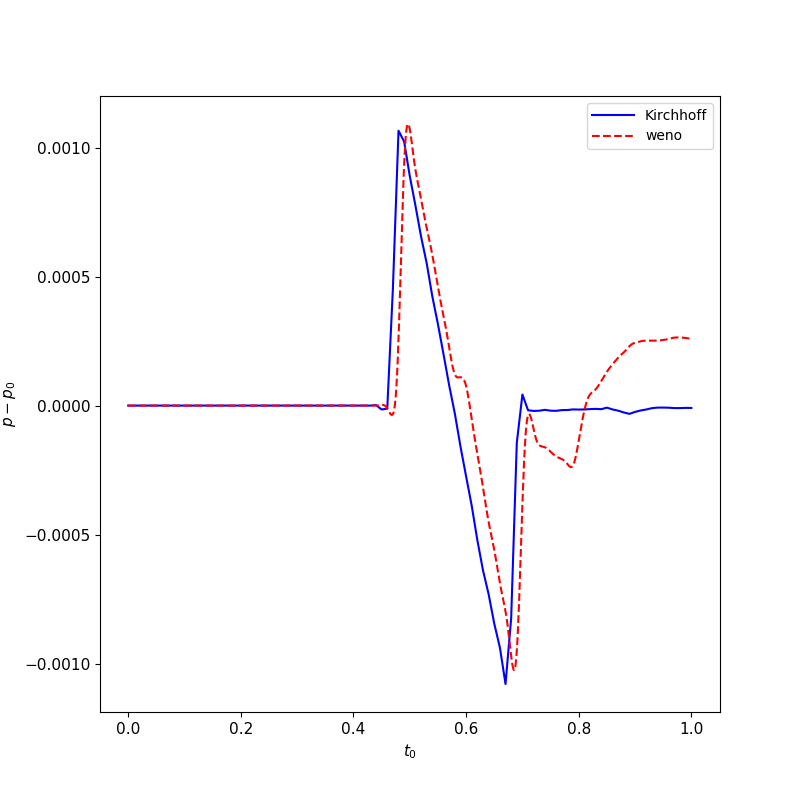
\includegraphics[scale=.7]{images/Pressure.png}
	\caption{The acoustic pressure $p' = p - p_{0}$ is computed at observer point $x_{0}$ using Euler and Kirchhoff solver and plotted against observer time $t_{0}$.}
\end{figure}
\printbibliography
\end{document}

